\documentclass{article}

\usepackage{graphics}
\usepackage{color}
\usepackage{verbatim}
\usepackage{amsthm}
\usepackage{amsmath}
\usepackage{amssymb}
\usepackage{graphicx}
\usepackage{esint}
\usepackage{tikz}
\usetikzlibrary{bayesnet}

\begin{document}
\thispagestyle{empty}
\centering
%\missingfigure{Factor graph for binary logistic regression. Just imagine by yourself for now.}
%\includegraphics[scale=0.8,page=2,clip,trim=8cm 18.5cm 8cm 1cm]{img/heess_passing_ep_supp.pdf}
%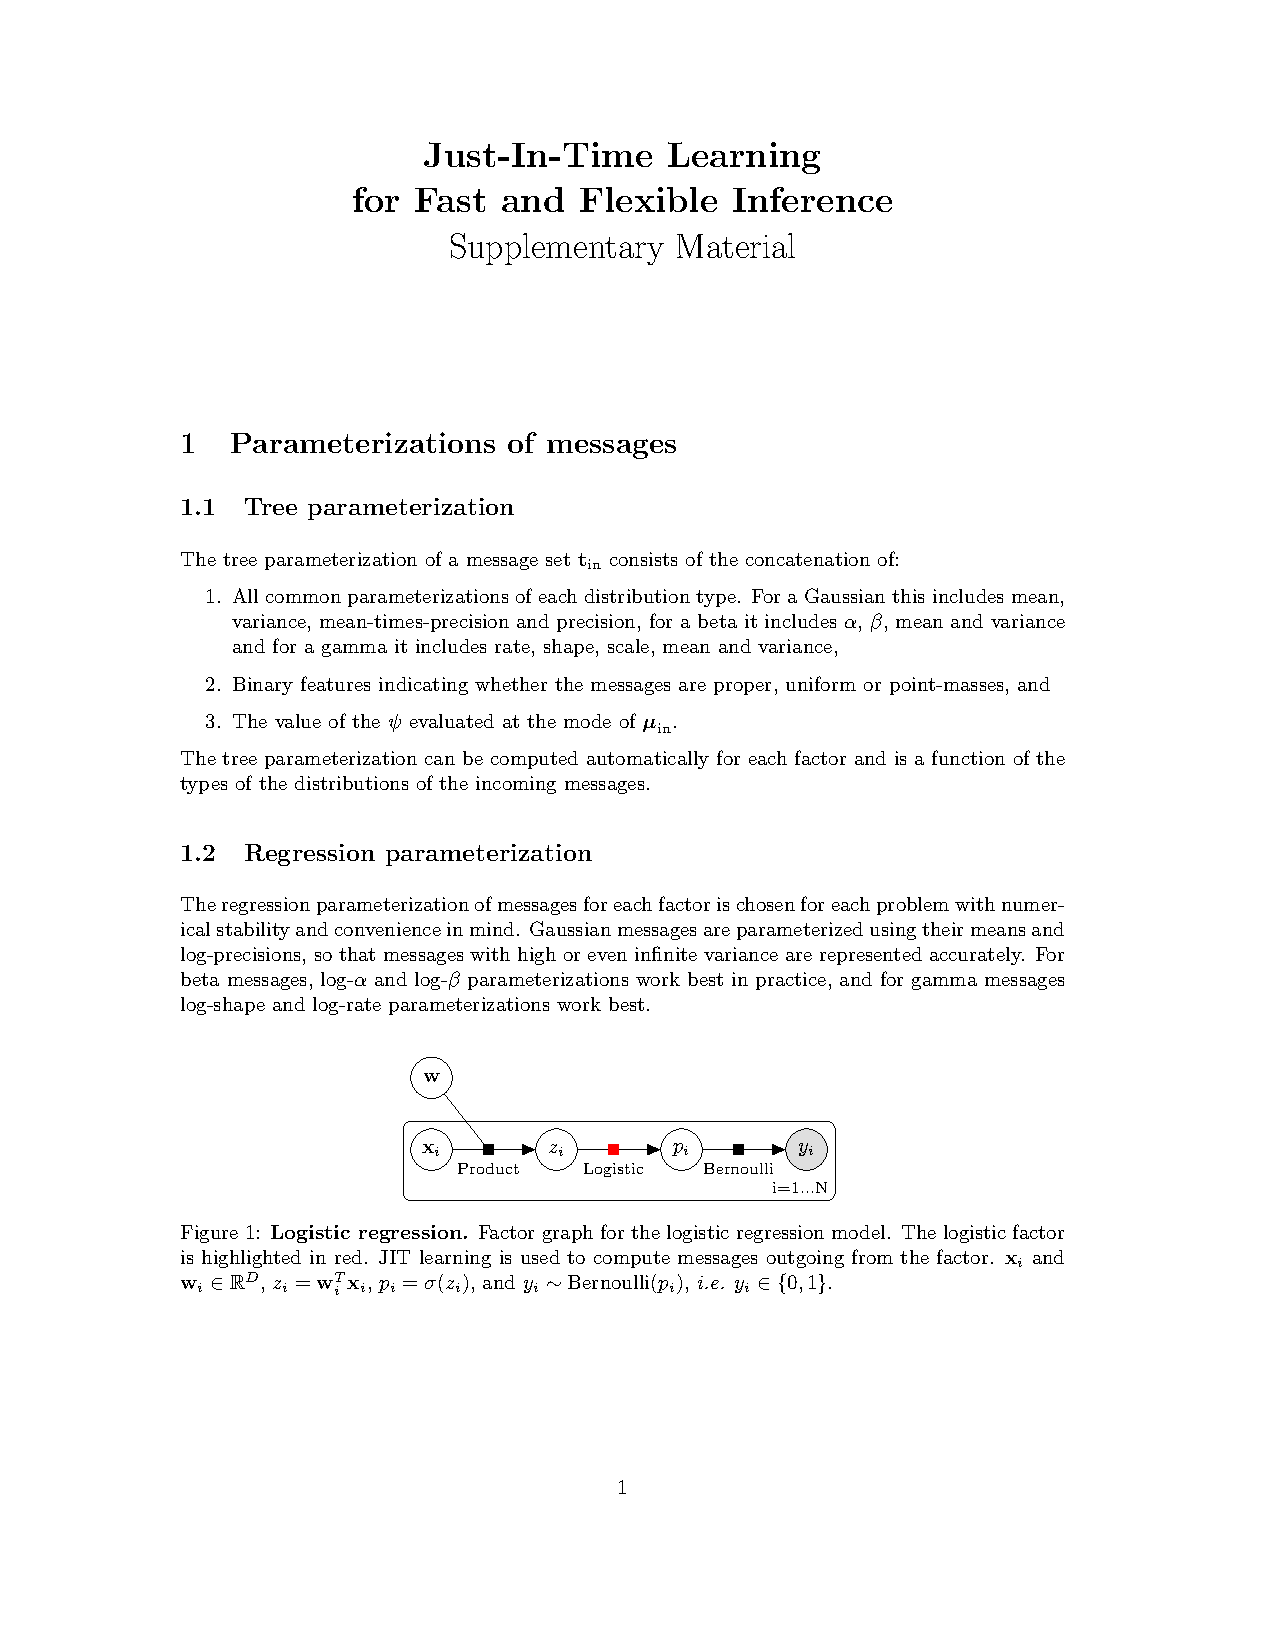
\includegraphics[scale=0.8,page=1,clip,trim=6.5cm 7.5cm 7cm 17.8cm]{img/eslami_jit_supp.pdf}
\begin{tikzpicture}
    \node (title) at (4.2, 1) {\large \textbf{Binary Logistic
    Regression}};
 \node[obs] (x) {$x_i$};
 \bayesfactor[right= of x] {dot} {below:dot} {} {};
 \node[latent, above = 5mm of dot] (w) {$\boldsymbol{w}$};
 \node[latent, right = 6mm of dot] (z) {$z_i$};
 \bayesfactor[right= 6mm of z, color=red] {logistic} {below:logistic ($f$)} {} {};
 \node[latent, right = 8mm of logistic] (p) {$p_i$};
 \bayesfactor[right = 6mm of p] {bern} {below:Bernoulli} {} {};
 \node[obs, right = 8mm of bern]  (y)   {$y_i$}; %
 
 \factoredge {x} {dot} {z};
 \factoredge {z} {logistic} {p};
 \factoredge {p} {bern} {y};
 
 
 \edge[-] {dot} {x} ;
 \edge[-] {w} {dot};
 \edge[-] {dot} {z} ;
 \edge[-] {z} {logistic} ;
 \edge[-] {logistic} {p};
 \edge[-] {p} {y} ;
 
  \plate {sample} { %
    (x)  (z) (p) (y)
  } {$i=1, \ldots, N$} ;
  
\end{tikzpicture}
\end{document}
